\section{Proposed Method}
\label{sec:method}

The architecture of HESOD is shown in Fig.~\ref{fig:overview}. From input $\mathbf{I} \in \mathbb{R}^{H \times W \times 3}$, a shallow stem extracts dense features $\mathbf{F} \in \mathbb{R}^{H_s \times W_s \times C}$. The \emph{Dual-Evidence Spatial Selector} then coordinates: (i) a priority head fusing semantic objectness with channel-pooled spectral saliency (Fig.~\ref{fig:overview}(b)) into spatial priority map $\mathbf{S} \in [0, 1]^{H_s \times W_s}$; and (ii) an AdaSlicer module (unchanged from ESOD~\cite{ESOD}) clustering candidate foreground cells into bounding patches $\mathcal{P}$. Downstream backbone stages and lightweight decoupled heads evaluate only retained patches $\mathcal{P}$, trained under the soft-coverage supervision (Sec.~\ref{ssec:coverage}) via the two-stage protocol (Sec.~\ref{ssec:head}).

\subsection{Dual-Evidence Priority Estimation}
\label{ssec:evidence}

To rescue micro targets with degraded semantic activations, HESOD couples high-level semantic confidence with low-level structural gradient saliency at negligible compute overhead (Fig.~\ref{fig:overview}(b)).

Let $\mathbf{f}_i \in \mathbb{R}^C$ denote the feature vector at spatial location $i$ in $\mathbf{F}$. The semantic branch predicts class-specific logits via a $1\times 1$ convolution: $\mathbf{z}^{\mathrm{sem}}_i = \mathrm{Conv}_{1\times 1}(\mathbf{f}_i) \in \mathbb{R}^{N_c}$. In parallel, the spectral branch extracts high-frequency structural gradients by first compressing channels via max- and mean-pooling:
\begin{equation}
\mathbf{F}_{\mathrm{pooled}} = \left[ \max_c \mathbf{F}_{:,:,c} \,\|\, \frac{1}{C}\sum_{c=1}^C \mathbf{F}_{:,:,c} \right] \in \mathbb{R}^{H_s \times W_s \times 2},
\label{eq:channel_pool}
\end{equation}
where $\mathbf{F}_{:,:,c} \in \mathbb{R}^{H_s \times W_s}$ is the $c$-th channel of $\mathbf{F}$ and $\|$ denotes channel-wise concatenation. Compressing $\mathbf{F}$ to 2 channels retains peak edge activation and background energy, after which a learnable depthwise $3\times 3$ convolution bank---initialized with discrete Laplacian and directional Sobel operators---filters $\mathbf{F}_{\mathrm{pooled}}$ into 6 structural channels at $\mathcal{O}(H_s W_s)$ cost independent of width $C$. In the 2D spatial frequency domain, the discrete Laplacian is approximately isotropic in the low-frequency limit, with $|H(\mathbf{\omega})| \propto \|\mathbf{\omega}\|^2$, naturally amplifying edge transitions. Because micro targets (\textless$16^2$\,px) manifest as localized high-frequency spatial impulses whose gradient energy resists downsampling~\cite{Zhao2025TGRS}, this branch supplies a constant-width prior independent of deep semantic capacity. A $1\times 1$ projection maps features to $N_c$, yielding spectral logits $\mathbf{z}^{\mathrm{spec}}_i \in \mathbb{R}^{N_c}$.

To prevent confidence dilution on faint targets, evidence fusion enforces \emph{evidence preservation}. Linear combinations risk destructive interference: an unconfident or negative activation in one branch can drag down a confident signal in the other below the routing threshold. Instead, we formulate a parameter-free elementwise maximum:
\begin{equation}
z_{i,c} = \max\!\left(z^{\mathrm{sem}}_{i,c},\, z^{\mathrm{spec}}_{i,c}\right), \quad s_i = \max_{c=1}^{N_c} \sigma(z_{i,c}),
\label{eq:fusion}
\end{equation}
This operation functions as an evidence-preserving OR gate: since $z_{i,c} \ge z^{\mathrm{sem}}_{i,c}$ and $z_{i,c} \ge z^{\mathrm{spec}}_{i,c}$, neither branch can ever suppress genuine candidate cues. Cells with priority $s_i > \tau$ are clustered into bounding patches $\mathcal{P}$ for downstream detection.

\subsection{Object-Level Soft-Coverage Loss}
\label{ssec:coverage}

Standard pixel-wise binary cross-entropy (BCE) evaluates grid cells independently, failing to guarantee instance-level coverage: a selector may over-allocate cells to large objects while dropping micro objects whose receptive fields contain only weak responses. To prevent premature false negatives, we formulate a differentiable object-level soft-coverage loss.

Let $\mathcal{N}(j)$ denote the set of selector cells overlapping ground-truth box $j \in \{1, \dots, N_{\mathrm{gt}}\}$. We formulate a noisy-OR differentiable coverage surrogate and its weighted instance loss:
\begin{equation}
p_j^{\mathrm{cover}} = 1 - \prod_{i \in \mathcal{N}(j)} (1 - s_i), \quad \ell_j = -w_j \log\left( p_j^{\mathrm{cover}} + \epsilon \right),
\label{eq:cover_loss}
\end{equation}
where $w_j = \operatorname{clip}(4/a_j, 1, 5)$ is a scale-adaptive weight based on bounding box area $a_j$ in cells, penalizing misses on micro targets ($a_j < 4$). For any cell $i \in \mathcal{N}(j)$, the gradient of $\ell_j$ with respect to cell score $s_i$ is:
\begin{equation}
\frac{\partial \ell_j}{\partial s_i} = -\frac{w_j}{p_j^{\mathrm{cover}} + \epsilon} \prod_{k \in \mathcal{N}(j) \setminus \{i\}} (1 - s_k).
\label{eq:cover_grad}
\end{equation}
When neighboring candidate cells have low scores ($s_k \to 0$), the product term approaches $1$, generating a strong gradient to boost cell $i$ and encouraging at least one cell to activate per instance. The overall soft-coverage loss averages over instances: $\mathcal{L}_{\mathrm{cover}} = \frac{1}{N_{\mathrm{gt}}} \sum_{j=1}^{N_{\mathrm{gt}}} \ell_j$. The multi-task training objective is $\mathcal{L} = \mathcal{L}_{\mathrm{det}} + \lambda_{\mathrm{sel}}(\mathcal{L}_{\mathrm{BCE}} + \lambda_{\mathrm{cov}}\mathcal{L}_{\mathrm{cover}})$, where $\mathcal{L}_{\mathrm{BCE}}$ is the per-cell selector BCE over scores $s_i$, with $\lambda_{\mathrm{sel}}=0.2$ and $\lambda_{\mathrm{cov}}=0.5$.

\subsection{Lightweight Decoupled Head and Training Protocol}
\label{ssec:head}

\begin{figure}[t]
\centering
\vspace{-1mm}
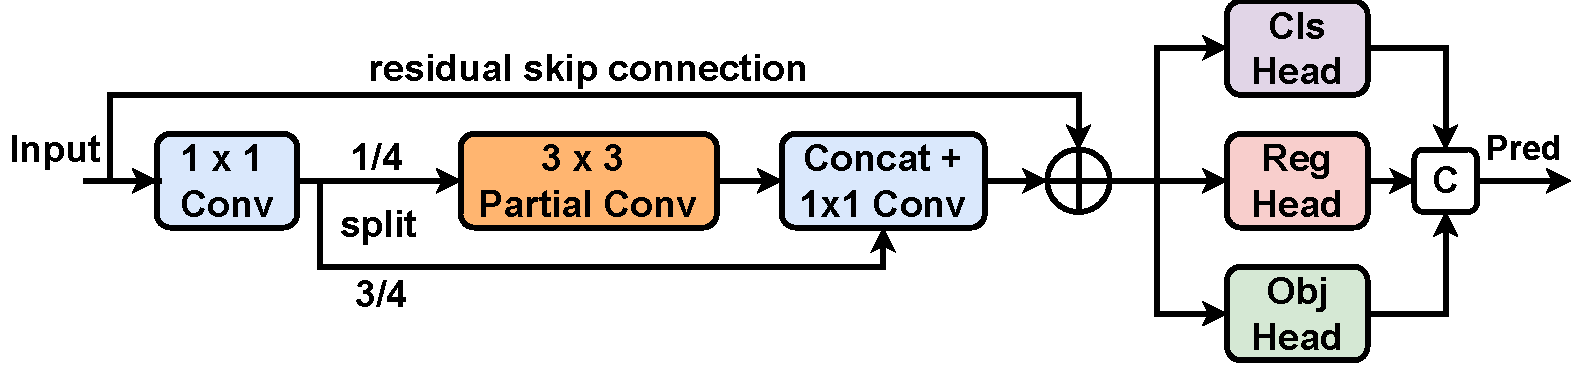
\includegraphics[width=\columnwidth]{figures/ISPPHead.pdf}
\vspace{-6mm}
\caption{Inverse-Residual Shared-Parameter Partial-Convolution (ISPP) Head (\textcircled{\scriptsize C} denotes channel concatenation).}
\label{fig:ispphead}
\vspace{7pt}
\end{figure}

While dual-evidence routing substantially improves patch coverage by retaining faint foreground regions, evaluating more candidate patches increases downstream detector computation. To recover this overhead without sacrificing selector gains, HESOD incorporates an ISPP decoupled head~\cite{ESODYOLO} as a dedicated compute compensator.

As shown in Fig.~\ref{fig:ispphead}, the ISPP head expands neck feature channels of width $C_1$ to $2C_1$, partitioning them into an active branch ($0.25$ ratio) processed by a $3\times 3$ Partial Convolution (PConv) and an identity passthrough branch ($0.75$ ratio). After linear projection and residual addition, decoupled $1\times 1$ heads predict classification, box regression, and objectness independently, lowering arithmetic complexity while eliminating inter-task gradient interference.

\textbf{Two-Stage Training Protocol.} To ensure stable routing behavior, HESOD employs a two-stage training scheme: (i)~\emph{Stage 1 (Selector Convergence)}: Train the Dual-Max selector with a coupled head under $\mathcal{L}_{\mathrm{cover}}$, establishing a well-calibrated priority heatmap; and (ii)~\emph{Stage 2 (Head Fine-Tuning)}: Freeze the upstream trunk (backbone, dual branches, router) and fine-tune the lightweight ISPP neck and decoupled heads on the frozen routing distribution. Relative to the uncompressed Dual-Max selector, this lightweight head slashes GFLOPs by 16.9\% and parameters by 27.5\% (on UAVDT) while fully preserving peak selector coverage (0.940), maintaining competitive real-time FPS with only fractional FLOPs overhead vs.~ESOD.

